\documentclass[twoside]{book}

% Packages required by doxygen
\usepackage{fixltx2e}
\usepackage{calc}
\usepackage{doxygen}
\usepackage[export]{adjustbox} % also loads graphicx
\usepackage{graphicx}
\usepackage[utf8]{inputenc}
\usepackage{makeidx}
\usepackage{multicol}
\usepackage{multirow}
\PassOptionsToPackage{warn}{textcomp}
\usepackage{textcomp}
\usepackage[nointegrals]{wasysym}
\usepackage[table]{xcolor}

% Font selection
\usepackage[T1]{fontenc}
\usepackage[scaled=.90]{helvet}
\usepackage{courier}
\usepackage{amssymb}
\usepackage{sectsty}
\renewcommand{\familydefault}{\sfdefault}
\allsectionsfont{%
  \fontseries{bc}\selectfont%
  \color{darkgray}%
}
\renewcommand{\DoxyLabelFont}{%
  \fontseries{bc}\selectfont%
  \color{darkgray}%
}
\newcommand{\+}{\discretionary{\mbox{\scriptsize$\hookleftarrow$}}{}{}}

% Page & text layout
\usepackage{geometry}
\geometry{%
  a4paper,%
  top=2.5cm,%
  bottom=2.5cm,%
  left=2.5cm,%
  right=2.5cm%
}
\tolerance=750
\hfuzz=15pt
\hbadness=750
\setlength{\emergencystretch}{15pt}
\setlength{\parindent}{0cm}
\setlength{\parskip}{3ex plus 2ex minus 2ex}
\makeatletter
\renewcommand{\paragraph}{%
  \@startsection{paragraph}{4}{0ex}{-1.0ex}{1.0ex}{%
    \normalfont\normalsize\bfseries\SS@parafont%
  }%
}
\renewcommand{\subparagraph}{%
  \@startsection{subparagraph}{5}{0ex}{-1.0ex}{1.0ex}{%
    \normalfont\normalsize\bfseries\SS@subparafont%
  }%
}
\makeatother

% Headers & footers
\usepackage{fancyhdr}
\pagestyle{fancyplain}
\fancyhead[LE]{\fancyplain{}{\bfseries\thepage}}
\fancyhead[CE]{\fancyplain{}{}}
\fancyhead[RE]{\fancyplain{}{\bfseries\leftmark}}
\fancyhead[LO]{\fancyplain{}{\bfseries\rightmark}}
\fancyhead[CO]{\fancyplain{}{}}
\fancyhead[RO]{\fancyplain{}{\bfseries\thepage}}
\fancyfoot[LE]{\fancyplain{}{}}
\fancyfoot[CE]{\fancyplain{}{}}
\fancyfoot[RE]{\fancyplain{}{\bfseries\scriptsize Generated by Doxygen }}
\fancyfoot[LO]{\fancyplain{}{\bfseries\scriptsize Generated by Doxygen }}
\fancyfoot[CO]{\fancyplain{}{}}
\fancyfoot[RO]{\fancyplain{}{}}
\renewcommand{\footrulewidth}{0.4pt}
\renewcommand{\chaptermark}[1]{%
  \markboth{#1}{}%
}
\renewcommand{\sectionmark}[1]{%
  \markright{\thesection\ #1}%
}

% Indices & bibliography
\usepackage{natbib}
\usepackage[titles]{tocloft}
\setcounter{tocdepth}{3}
\setcounter{secnumdepth}{5}
\makeindex

% Hyperlinks (required, but should be loaded last)
\usepackage{ifpdf}
\ifpdf
  \usepackage[pdftex,pagebackref=true]{hyperref}
\else
  \usepackage[ps2pdf,pagebackref=true]{hyperref}
\fi
\hypersetup{%
  colorlinks=true,%
  linkcolor=blue,%
  citecolor=blue,%
  unicode%
}

% Custom commands
\newcommand{\clearemptydoublepage}{%
  \newpage{\pagestyle{empty}\cleardoublepage}%
}

\usepackage{caption}
\captionsetup{labelsep=space,justification=centering,font={bf},singlelinecheck=off,skip=4pt,position=top}

%===== C O N T E N T S =====

\begin{document}

% Titlepage & ToC
\hypersetup{pageanchor=false,
             bookmarksnumbered=true,
             pdfencoding=unicode
            }
\pagenumbering{alph}
\begin{titlepage}
\vspace*{7cm}
\begin{center}%
{\Large S\+A\+E102 }\\
\vspace*{1cm}
{\large Generated by Doxygen 1.8.13}\\
\end{center}
\end{titlepage}
\clearemptydoublepage
\pagenumbering{roman}
\tableofcontents
\clearemptydoublepage
\pagenumbering{arabic}
\hypersetup{pageanchor=true}

%--- Begin generated contents ---
\chapter{Data Structure Index}
\section{Data Structures}
Here are the data structures with brief descriptions\+:\begin{DoxyCompactList}
\item\contentsline{section}{\hyperlink{struct_date}{Date} }{\pageref{struct_date}}{}
\item\contentsline{section}{\hyperlink{struct_date_dem}{Date\+Dem} }{\pageref{struct_date_dem}}{}
\item\contentsline{section}{\hyperlink{structliste_dem}{liste\+Dem} }{\pageref{structliste_dem}}{}
\item\contentsline{section}{\hyperlink{struct_locataire}{Locataire} }{\pageref{struct_locataire}}{}
\item\contentsline{section}{\hyperlink{struct_logement}{Logement} }{\pageref{struct_logement}}{}
\item\contentsline{section}{\hyperlink{structmaillonloc}{maillonloc} }{\pageref{structmaillonloc}}{}
\item\contentsline{section}{\hyperlink{struct_menage}{Menage} }{\pageref{struct_menage}}{}
\item\contentsline{section}{\hyperlink{struct_tel}{Tel} }{\pageref{struct_tel}}{}
\end{DoxyCompactList}

\chapter{File Index}
\section{File List}
Here is a list of all documented files with brief descriptions\+:\begin{DoxyCompactList}
\item\contentsline{section}{/home/\+I\+U\+T/thmuzard/\+Documents/\+S\+A\+E/\+N\+\_\+1.\+02/sae1.\+02/\+Code/{\bfseries hlm.\+h} }{\pageref{hlm_8h}}{}
\item\contentsline{section}{/home/\+I\+U\+T/thmuzard/\+Documents/\+S\+A\+E/\+N\+\_\+1.\+02/sae1.\+02/\+Code/\hyperlink{hlm_demandeur_8c}{hlm\+Demandeur.\+c} \\*Emsemble des fonctions permettant de gérés la partit sur les demandes de logement  V\+E\+R\+D\+I\+ER Nathan, M\+U\+Z\+A\+RD Thomas }{\pageref{hlm_demandeur_8c}}{}
\item\contentsline{section}{/home/\+I\+U\+T/thmuzard/\+Documents/\+S\+A\+E/\+N\+\_\+1.\+02/sae1.\+02/\+Code/\hyperlink{hlm_logement_8c}{hlm\+Logement.\+c} \\*Ce fichier contiendra l\textquotesingle{}ensemble des fonction nécessaire au traitement des logement de la société }{\pageref{hlm_logement_8c}}{}
\item\contentsline{section}{/home/\+I\+U\+T/thmuzard/\+Documents/\+S\+A\+E/\+N\+\_\+1.\+02/sae1.\+02/\+Code/\hyperlink{menu_8c}{menu.\+c} \\*Dans cette partie du programme, nous traitons les fonctions d\textquotesingle{}affichage des menu et l\textquotesingle{}aspect visuel du code. C\textquotesingle{}est ici que nous allons appellé toutes nos fonctions }{\pageref{menu_8c}}{}
\end{DoxyCompactList}

\chapter{Data Structure Documentation}
\hypertarget{struct_date}{}\section{Date Struct Reference}
\label{struct_date}\index{Date@{Date}}
\subsection*{Data Fields}
\begin{DoxyCompactItemize}
\item 
\mbox{\Hypertarget{struct_date_a14cfca53638083a91dc9d133a57126d1}\label{struct_date_a14cfca53638083a91dc9d133a57126d1}} 
int {\bfseries jours}
\item 
\mbox{\Hypertarget{struct_date_af4d47133f30c1a134b6cecf5cedd7db9}\label{struct_date_af4d47133f30c1a134b6cecf5cedd7db9}} 
int {\bfseries mois}
\item 
\mbox{\Hypertarget{struct_date_acfe2ff64f5396827db36f1575c5e99d8}\label{struct_date_acfe2ff64f5396827db36f1575c5e99d8}} 
int {\bfseries annee}
\end{DoxyCompactItemize}


The documentation for this struct was generated from the following file\+:\begin{DoxyCompactItemize}
\item 
/home/\+I\+U\+T/thmuzard/\+Documents/\+S\+A\+E/\+N\+\_\+1.\+02/sae1.\+02/\+Code/hlm.\+h\end{DoxyCompactItemize}

\hypertarget{struct_date_dem}{}\section{Date\+Dem Struct Reference}
\label{struct_date_dem}\index{Date\+Dem@{Date\+Dem}}
\subsection*{Data Fields}
\begin{DoxyCompactItemize}
\item 
\mbox{\Hypertarget{struct_date_dem_a14cfca53638083a91dc9d133a57126d1}\label{struct_date_dem_a14cfca53638083a91dc9d133a57126d1}} 
int {\bfseries jours}
\item 
\mbox{\Hypertarget{struct_date_dem_af4d47133f30c1a134b6cecf5cedd7db9}\label{struct_date_dem_af4d47133f30c1a134b6cecf5cedd7db9}} 
int {\bfseries mois}
\item 
\mbox{\Hypertarget{struct_date_dem_acfe2ff64f5396827db36f1575c5e99d8}\label{struct_date_dem_acfe2ff64f5396827db36f1575c5e99d8}} 
int {\bfseries annee}
\item 
\mbox{\Hypertarget{struct_date_dem_af109a7090a39da6ff71d5c31dbde1e09}\label{struct_date_dem_af109a7090a39da6ff71d5c31dbde1e09}} 
int {\bfseries heure}
\item 
\mbox{\Hypertarget{struct_date_dem_a5edffad982a0566ad01d95005474eae3}\label{struct_date_dem_a5edffad982a0566ad01d95005474eae3}} 
int {\bfseries minute}
\item 
\mbox{\Hypertarget{struct_date_dem_acc9b185ad0fb0cdebb456ba26fa2828d}\label{struct_date_dem_acc9b185ad0fb0cdebb456ba26fa2828d}} 
int {\bfseries seconde}
\end{DoxyCompactItemize}


The documentation for this struct was generated from the following file\+:\begin{DoxyCompactItemize}
\item 
/home/\+I\+U\+T/thmuzard/\+Documents/\+S\+A\+E/\+N\+\_\+1.\+02/sae1.\+02/\+Code/hlm.\+h\end{DoxyCompactItemize}

\hypertarget{structliste_dem}{}\section{liste\+Dem Struct Reference}
\label{structliste_dem}\index{liste\+Dem@{liste\+Dem}}


Collaboration diagram for liste\+Dem\+:
\nopagebreak
\begin{figure}[H]
\begin{center}
\leavevmode
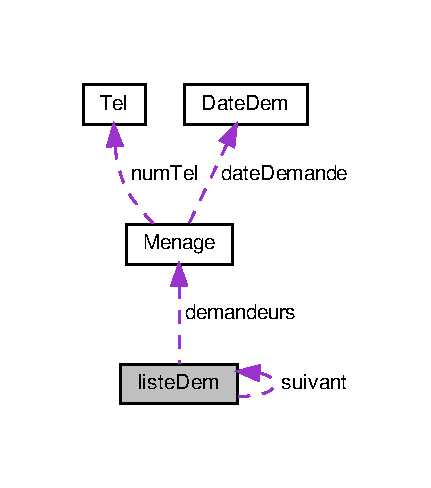
\includegraphics[width=207pt]{structliste_dem__coll__graph}
\end{center}
\end{figure}
\subsection*{Data Fields}
\begin{DoxyCompactItemize}
\item 
\mbox{\Hypertarget{structliste_dem_a76e6c62c1b79181ed799adda3abf7ddb}\label{structliste_dem_a76e6c62c1b79181ed799adda3abf7ddb}} 
\hyperlink{struct_menage}{Menage} {\bfseries demandeurs}
\item 
\mbox{\Hypertarget{structliste_dem_a8c4767137afdf35dde77dc1b9d27dfd2}\label{structliste_dem_a8c4767137afdf35dde77dc1b9d27dfd2}} 
struct \hyperlink{structliste_dem}{liste\+Dem} $\ast$ {\bfseries suivant}
\end{DoxyCompactItemize}


The documentation for this struct was generated from the following file\+:\begin{DoxyCompactItemize}
\item 
/home/\+I\+U\+T/thmuzard/\+Documents/\+S\+A\+E/\+N\+\_\+1.\+02/sae1.\+02/\+Code/hlm.\+h\end{DoxyCompactItemize}

\hypertarget{struct_locataire}{}\section{Locataire Struct Reference}
\label{struct_locataire}\index{Locataire@{Locataire}}


Collaboration diagram for Locataire\+:
\nopagebreak
\begin{figure}[H]
\begin{center}
\leavevmode
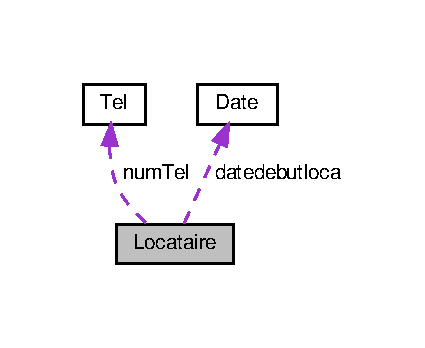
\includegraphics[width=204pt]{struct_locataire__coll__graph}
\end{center}
\end{figure}
\subsection*{Data Fields}
\begin{DoxyCompactItemize}
\item 
\mbox{\Hypertarget{struct_locataire_adc5a9bd2de6d5bb662f5c5828138669e}\label{struct_locataire_adc5a9bd2de6d5bb662f5c5828138669e}} 
int {\bfseries numloca}
\item 
\mbox{\Hypertarget{struct_locataire_ab12db00e8885e637d3ebd7b87adf564c}\label{struct_locataire_ab12db00e8885e637d3ebd7b87adf564c}} 
char {\bfseries prenom} \mbox{[}31\mbox{]}
\item 
\mbox{\Hypertarget{struct_locataire_a3d20d8a77afd57aa83185d38427aabfe}\label{struct_locataire_a3d20d8a77afd57aa83185d38427aabfe}} 
char {\bfseries nom} \mbox{[}31\mbox{]}
\item 
\mbox{\Hypertarget{struct_locataire_ad5bc5a64fd7ac927b2a45cd4dcf7af62}\label{struct_locataire_ad5bc5a64fd7ac927b2a45cd4dcf7af62}} 
char {\bfseries nationalite} \mbox{[}3\mbox{]}
\item 
\mbox{\Hypertarget{struct_locataire_ae7089f702bde28e49c864a37138a0e8a}\label{struct_locataire_ae7089f702bde28e49c864a37138a0e8a}} 
int {\bfseries plafond}
\item 
\mbox{\Hypertarget{struct_locataire_a18d355c50be82ddec8de8dfa65a09a9e}\label{struct_locataire_a18d355c50be82ddec8de8dfa65a09a9e}} 
float {\bfseries revenu}
\item 
\mbox{\Hypertarget{struct_locataire_aff8364c2d38c1568a70e844a92f049c0}\label{struct_locataire_aff8364c2d38c1568a70e844a92f049c0}} 
int {\bfseries numlogement}
\item 
\mbox{\Hypertarget{struct_locataire_ad4bbf90506e48b5c4701d68ae5420238}\label{struct_locataire_ad4bbf90506e48b5c4701d68ae5420238}} 
float {\bfseries prix\+Log}
\item 
\mbox{\Hypertarget{struct_locataire_ad0c32e07f1ab6af999703d5e60ef3e60}\label{struct_locataire_ad0c32e07f1ab6af999703d5e60ef3e60}} 
int {\bfseries nb\+Num\+Tel}
\item 
\mbox{\Hypertarget{struct_locataire_af6fcbb8b18e974fd8bca72a528955a51}\label{struct_locataire_af6fcbb8b18e974fd8bca72a528955a51}} 
\hyperlink{struct_tel}{Tel} $\ast$ {\bfseries num\+Tel}
\item 
\mbox{\Hypertarget{struct_locataire_af79ff191ea30744d721b46dacd5f9ff3}\label{struct_locataire_af79ff191ea30744d721b46dacd5f9ff3}} 
\hyperlink{struct_date}{Date} {\bfseries datedebutloca}
\end{DoxyCompactItemize}


The documentation for this struct was generated from the following file\+:\begin{DoxyCompactItemize}
\item 
/home/\+I\+U\+T/thmuzard/\+Documents/\+S\+A\+E/\+N\+\_\+1.\+02/sae1.\+02/\+Code/hlm.\+h\end{DoxyCompactItemize}

\hypertarget{struct_logement}{}\section{Logement Struct Reference}
\label{struct_logement}\index{Logement@{Logement}}


Collaboration diagram for Logement\+:
\nopagebreak
\begin{figure}[H]
\begin{center}
\leavevmode
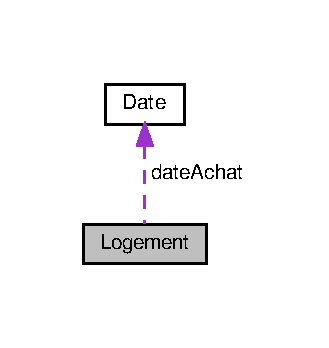
\includegraphics[width=158pt]{struct_logement__coll__graph}
\end{center}
\end{figure}
\subsection*{Data Fields}
\begin{DoxyCompactItemize}
\item 
\mbox{\Hypertarget{struct_logement_ad8bc1cf03e6bd5d3a06df1de9830ef88}\label{struct_logement_ad8bc1cf03e6bd5d3a06df1de9830ef88}} 
int {\bfseries num\+Logement}
\item 
\mbox{\Hypertarget{struct_logement_a03c7718814cc87682a5d2dfce7b287d7}\label{struct_logement_a03c7718814cc87682a5d2dfce7b287d7}} 
char {\bfseries type\+Log} \mbox{[}3\mbox{]}
\item 
\mbox{\Hypertarget{struct_logement_a5e44ddbcd31c92ef9fbc26c68cbdd85b}\label{struct_logement_a5e44ddbcd31c92ef9fbc26c68cbdd85b}} 
int {\bfseries nb\+Chambre}
\item 
\mbox{\Hypertarget{struct_logement_a669a792fad91b1d30d5abf3d0daf099a}\label{struct_logement_a669a792fad91b1d30d5abf3d0daf099a}} 
float {\bfseries surface\+Log}
\item 
\mbox{\Hypertarget{struct_logement_ad4bbf90506e48b5c4701d68ae5420238}\label{struct_logement_ad4bbf90506e48b5c4701d68ae5420238}} 
float {\bfseries prix\+Log}
\item 
\mbox{\Hypertarget{struct_logement_a53fba463f9f34aa7d8da0d0ea71fd5fe}\label{struct_logement_a53fba463f9f34aa7d8da0d0ea71fd5fe}} 
char {\bfseries dispo} \mbox{[}5\mbox{]}
\item 
\mbox{\Hypertarget{struct_logement_a530275c4532dc6044a2a1d4ddb835de3}\label{struct_logement_a530275c4532dc6044a2a1d4ddb835de3}} 
\hyperlink{struct_date}{Date} {\bfseries date\+Achat}
\end{DoxyCompactItemize}


The documentation for this struct was generated from the following file\+:\begin{DoxyCompactItemize}
\item 
/home/\+I\+U\+T/thmuzard/\+Documents/\+S\+A\+E/\+N\+\_\+1.\+02/sae1.\+02/\+Code/hlm.\+h\end{DoxyCompactItemize}

\hypertarget{structmaillonloc}{}\section{maillonloc Struct Reference}
\label{structmaillonloc}\index{maillonloc@{maillonloc}}


Collaboration diagram for maillonloc\+:
\nopagebreak
\begin{figure}[H]
\begin{center}
\leavevmode
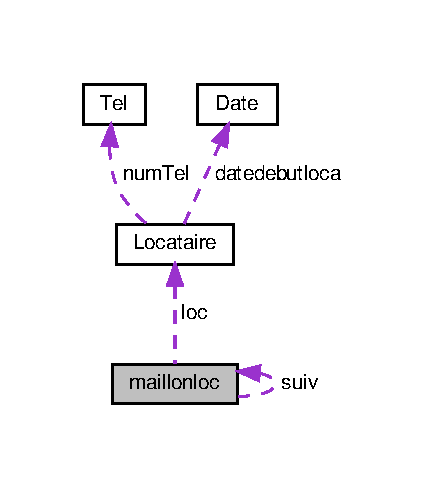
\includegraphics[width=204pt]{structmaillonloc__coll__graph}
\end{center}
\end{figure}
\subsection*{Data Fields}
\begin{DoxyCompactItemize}
\item 
\mbox{\Hypertarget{structmaillonloc_a93f86743307f08fbd6581318e23c0342}\label{structmaillonloc_a93f86743307f08fbd6581318e23c0342}} 
\hyperlink{struct_locataire}{Locataire} {\bfseries loc}
\item 
\mbox{\Hypertarget{structmaillonloc_a324f811e85c0a337dbc0ad4968d4d068}\label{structmaillonloc_a324f811e85c0a337dbc0ad4968d4d068}} 
struct \hyperlink{structmaillonloc}{maillonloc} $\ast$ {\bfseries suiv}
\end{DoxyCompactItemize}


The documentation for this struct was generated from the following file\+:\begin{DoxyCompactItemize}
\item 
/home/\+I\+U\+T/thmuzard/\+Documents/\+S\+A\+E/\+N\+\_\+1.\+02/sae1.\+02/\+Code/hlm.\+h\end{DoxyCompactItemize}

\hypertarget{struct_menage}{}\section{Menage Struct Reference}
\label{struct_menage}\index{Menage@{Menage}}


Collaboration diagram for Menage\+:
\nopagebreak
\begin{figure}[H]
\begin{center}
\leavevmode
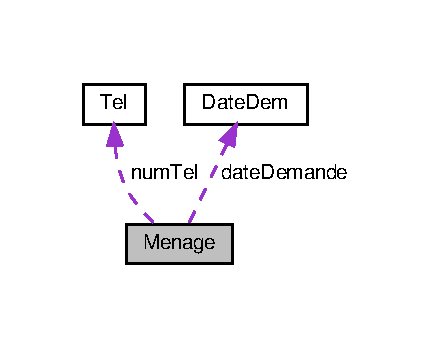
\includegraphics[width=207pt]{struct_menage__coll__graph}
\end{center}
\end{figure}
\subsection*{Data Fields}
\begin{DoxyCompactItemize}
\item 
\mbox{\Hypertarget{struct_menage_ac743b82b1da0e2bcf9ffaf0e9fd08034}\label{struct_menage_ac743b82b1da0e2bcf9ffaf0e9fd08034}} 
int {\bfseries num\+Demande}
\item 
\mbox{\Hypertarget{struct_menage_a0dc3b51805d54678be1c7ab3eebfe35f}\label{struct_menage_a0dc3b51805d54678be1c7ab3eebfe35f}} 
int {\bfseries nb\+Point}
\item 
\mbox{\Hypertarget{struct_menage_ae9237c6ce2605ffd02e67dd05202a6ff}\label{struct_menage_ae9237c6ce2605ffd02e67dd05202a6ff}} 
int {\bfseries nb\+Personne}
\item 
\mbox{\Hypertarget{struct_menage_a783290410bb7ec687a5b660ea9f80708}\label{struct_menage_a783290410bb7ec687a5b660ea9f80708}} 
float {\bfseries revenue\+Brut}
\item 
\mbox{\Hypertarget{struct_menage_a0fb012454f87cc4f6bf2e53440c51428}\label{struct_menage_a0fb012454f87cc4f6bf2e53440c51428}} 
char {\bfseries nom\+De\+Famille} \mbox{[}31\mbox{]}
\item 
\mbox{\Hypertarget{struct_menage_ab12db00e8885e637d3ebd7b87adf564c}\label{struct_menage_ab12db00e8885e637d3ebd7b87adf564c}} 
char {\bfseries prenom} \mbox{[}31\mbox{]}
\item 
\mbox{\Hypertarget{struct_menage_ad5bc5a64fd7ac927b2a45cd4dcf7af62}\label{struct_menage_ad5bc5a64fd7ac927b2a45cd4dcf7af62}} 
char {\bfseries nationalite} \mbox{[}3\mbox{]}
\item 
\mbox{\Hypertarget{struct_menage_a16a1079c7488fd3a6df04e542b01bf72}\label{struct_menage_a16a1079c7488fd3a6df04e542b01bf72}} 
int {\bfseries nb\+Num}
\item 
\mbox{\Hypertarget{struct_menage_af6fcbb8b18e974fd8bca72a528955a51}\label{struct_menage_af6fcbb8b18e974fd8bca72a528955a51}} 
\hyperlink{struct_tel}{Tel} $\ast$ {\bfseries num\+Tel}
\item 
\mbox{\Hypertarget{struct_menage_a4aa620f84fe6a8e15b9592f7075ef8e2}\label{struct_menage_a4aa620f84fe6a8e15b9592f7075ef8e2}} 
\hyperlink{struct_date_dem}{Date\+Dem} {\bfseries date\+Demande}
\end{DoxyCompactItemize}


The documentation for this struct was generated from the following file\+:\begin{DoxyCompactItemize}
\item 
/home/\+I\+U\+T/thmuzard/\+Documents/\+S\+A\+E/\+N\+\_\+1.\+02/sae1.\+02/\+Code/hlm.\+h\end{DoxyCompactItemize}

\hypertarget{struct_tel}{}\section{Tel Struct Reference}
\label{struct_tel}\index{Tel@{Tel}}
\subsection*{Data Fields}
\begin{DoxyCompactItemize}
\item 
\mbox{\Hypertarget{struct_tel_a01e5e3ac06edf7784f94903394f5a1f2}\label{struct_tel_a01e5e3ac06edf7784f94903394f5a1f2}} 
char {\bfseries libelle} \mbox{[}30\mbox{]}
\item 
\mbox{\Hypertarget{struct_tel_a9e01a711cb30303f26a3e87ae68ebc02}\label{struct_tel_a9e01a711cb30303f26a3e87ae68ebc02}} 
char {\bfseries num} \mbox{[}15\mbox{]}
\end{DoxyCompactItemize}


The documentation for this struct was generated from the following file\+:\begin{DoxyCompactItemize}
\item 
/home/\+I\+U\+T/thmuzard/\+Documents/\+S\+A\+E/\+N\+\_\+1.\+02/sae1.\+02/\+Code/hlm.\+h\end{DoxyCompactItemize}

\chapter{File Documentation}
\hypertarget{hlm_demandeur_8c}{}\section{/home/\+I\+U\+T/thmuzard/\+Documents/\+S\+A\+E/\+N\+\_\+1.02/sae1.02/\+Code/hlm\+Demandeur.c File Reference}
\label{hlm_demandeur_8c}\index{/home/\+I\+U\+T/thmuzard/\+Documents/\+S\+A\+E/\+N\+\_\+1.\+02/sae1.\+02/\+Code/hlm\+Demandeur.\+c@{/home/\+I\+U\+T/thmuzard/\+Documents/\+S\+A\+E/\+N\+\_\+1.\+02/sae1.\+02/\+Code/hlm\+Demandeur.\+c}}


Emsemble des fonctions permettant de gérés la partit sur les demandes de logement  V\+E\+R\+D\+I\+ER Nathan, M\+U\+Z\+A\+RD Thomas.  


{\ttfamily \#include \char`\"{}hlm.\+h\char`\"{}}\newline
{\ttfamily \#include $<$stdio.\+h$>$}\newline
{\ttfamily \#include $<$stdlib.\+h$>$}\newline
{\ttfamily \#include $<$string.\+h$>$}\newline
Include dependency graph for hlm\+Demandeur.\+c\+:
\nopagebreak
\begin{figure}[H]
\begin{center}
\leavevmode
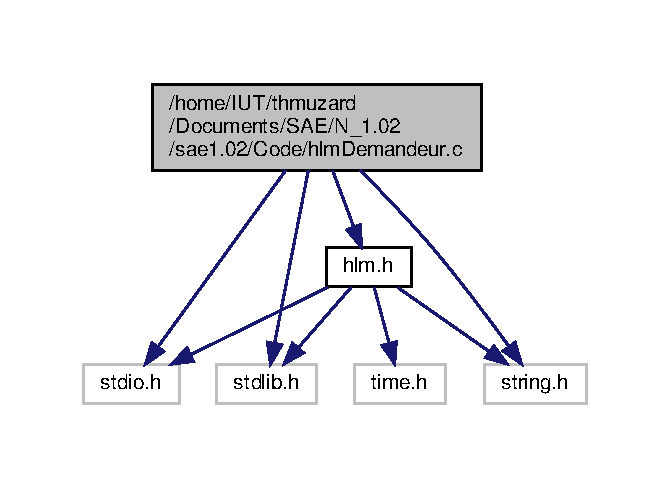
\includegraphics[width=322pt]{hlm_demandeur_8c__incl}
\end{center}
\end{figure}
\subsection*{Functions}
\begin{DoxyCompactItemize}
\item 
\hyperlink{structliste_dem}{Liste\+Dem} \hyperlink{hlm_demandeur_8c_a8385d4f84473a3ea06e9b8f60fa8d77d}{initliste} (void)
\begin{DoxyCompactList}\small\item\em initialisation de la liste \end{DoxyCompactList}\item 
\hyperlink{structliste_dem}{Liste\+Dem} \hyperlink{hlm_demandeur_8c_a9fdf732df5aea07cb07cbd637bacfd33}{lire\+Menage} (F\+I\+LE $\ast$f\+Dem, \hyperlink{structliste_dem}{Liste\+Dem} l)
\item 
\hyperlink{structliste_dem}{Liste\+Dem} \hyperlink{hlm_demandeur_8c_af72bde9e84d9e7ed8f3923a22a569c47}{chargement\+Dem} (\hyperlink{structliste_dem}{Liste\+Dem} l, int $\ast$nbD, char $\ast$fic)
\begin{DoxyCompactList}\small\item\em chargement demandeurs \end{DoxyCompactList}\item 
void \hyperlink{hlm_demandeur_8c_a21a25e6eaf315a4da600893384abd755}{affichage\+Dem} (\hyperlink{structliste_dem}{Liste\+Dem} l)
\begin{DoxyCompactList}\small\item\em Affichage liste demandeurs. \end{DoxyCompactList}\item 
void \hyperlink{hlm_demandeur_8c_a1abe63de7bd7191bf6b27501b682f594}{affichage\+Un\+Dem} (\hyperlink{structliste_dem}{Liste\+Dem} l)
\begin{DoxyCompactList}\small\item\em Affiche un seul demandeurs. \end{DoxyCompactList}\item 
\hyperlink{structliste_dem}{Liste\+Dem} \hyperlink{hlm_demandeur_8c_a3e870a67ffe71e156d00a80ae55c7ff5}{expiration\+Dem} (\hyperlink{structliste_dem}{Liste\+Dem} l, int $\ast$nbD)
\begin{DoxyCompactList}\small\item\em Supprime un demandeurs ayant fait une demande dépassant les 1 an. \end{DoxyCompactList}\item 
\hyperlink{structliste_dem}{Liste\+Dem} \hyperlink{hlm_demandeur_8c_aac8a31f60eb025f149664b2d4dd51952}{expiration\+Dem\+En\+Tete} (\hyperlink{structliste_dem}{Liste\+Dem} l, int $\ast$nbD)
\begin{DoxyCompactList}\small\item\em Supprime un demandeurs en tête. \end{DoxyCompactList}\item 
\hyperlink{structliste_dem}{Liste\+Dem} \hyperlink{hlm_demandeur_8c_a45506a0e114f12144a188ca436072f9b}{insertion\+En\+Tete\+Dem} (\hyperlink{structliste_dem}{Liste\+Dem} l, int num\+Demande, int nb\+Point, int nb\+Personne, float revenue\+Brut, char $\ast$nom\+De\+Famille, char $\ast$prenom, char $\ast$nationalite)
\begin{DoxyCompactList}\small\item\em Insère en tête de liste un demandeurs. \end{DoxyCompactList}\item 
Booleen \hyperlink{hlm_demandeur_8c_ae4cc1c3c6faac9d006cd5b08f2b755b4}{num\+Existe} (\hyperlink{structliste_dem}{Liste\+Dem} l, int value)
\begin{DoxyCompactList}\small\item\em Regarde si le numéro de demandeurs existe. \end{DoxyCompactList}\item 
\hyperlink{structliste_dem}{Liste\+Dem} \hyperlink{hlm_demandeur_8c_a7486cc07597951620be668805707f3b4}{recherche\+Un\+Demandeur} (\hyperlink{structliste_dem}{Liste\+Dem} l, int value)
\begin{DoxyCompactList}\small\item\em recherche un demandeurs dans la liste \end{DoxyCompactList}\item 
\hyperlink{structliste_dem}{Liste\+Dem} \hyperlink{hlm_demandeur_8c_a0f0049984a799fab42efa8890b5e8927}{insertion\+Dem} (\hyperlink{structliste_dem}{Liste\+Dem} l, int num\+Demande, int nb\+Point, int nb\+Personne, float revenue\+Brut, char $\ast$nom\+De\+Famille, char $\ast$prenom, char $\ast$nationalite)
\begin{DoxyCompactList}\small\item\em insère dans la liste un demandeurs \end{DoxyCompactList}\item 
void \hyperlink{hlm_demandeur_8c_a2770e35ecb9bb4b34ca7d983b24d7c50}{afficher\+Un\+Demandeur} (\hyperlink{structliste_dem}{Liste\+Dem} l, int value)
\begin{DoxyCompactList}\small\item\em Affiche un demandeur. \end{DoxyCompactList}\item 
\hyperlink{structliste_dem}{Liste\+Dem} \hyperlink{hlm_demandeur_8c_a55c499731ff81ad37d8546412b11f339}{suppression\+En\+Tete} (\hyperlink{structliste_dem}{Liste\+Dem} l, int $\ast$nbD)
\begin{DoxyCompactList}\small\item\em Supprime un élément en tête de liste. \end{DoxyCompactList}\item 
\hyperlink{structliste_dem}{Liste\+Dem} \hyperlink{hlm_demandeur_8c_a718c1ddf436a39504743664c581dd7d1}{suppression} (\hyperlink{structliste_dem}{Liste\+Dem} l, int supp\+Dem, int $\ast$nbD)
\begin{DoxyCompactList}\small\item\em Supprime un élément de la liste. \end{DoxyCompactList}\item 
void \hyperlink{hlm_demandeur_8c_afedcc74773cec58a7117f0a92a8368c1}{suppression\+All} (\hyperlink{structliste_dem}{Liste\+Dem} l, int $\ast$nbD)
\begin{DoxyCompactList}\small\item\em Supprime tout les éléments du fichier. \end{DoxyCompactList}\item 
\hyperlink{structliste_dem}{Liste\+Dem} \hyperlink{hlm_demandeur_8c_af91fa1d4c92b908726ea06eb44d81919}{modification\+En\+Tete} (\hyperlink{structliste_dem}{Liste\+Dem} l)
\begin{DoxyCompactList}\small\item\em Modification d\textquotesingle{}une demande en tête de liste. \end{DoxyCompactList}\item 
\hyperlink{structliste_dem}{Liste\+Dem} \hyperlink{hlm_demandeur_8c_a9b74cb8f1256628fdf3af031144c1462}{modification} (\hyperlink{structliste_dem}{Liste\+Dem} l, int modif)
\begin{DoxyCompactList}\small\item\em Modifie les informations d\textquotesingle{}une demande de logement dans la liste. \end{DoxyCompactList}\item 
void \hyperlink{hlm_demandeur_8c_a3e4f6c04636bd6890b5969dee1b1fed9}{sauvegarde\+Dem} (\hyperlink{structliste_dem}{Liste\+Dem} l, F\+I\+LE $\ast$f\+Dem)
\begin{DoxyCompactList}\small\item\em Sauvegarde dans le fichier l\textquotesingle{}ajout ou la modification d\textquotesingle{}une demandes de logement. \end{DoxyCompactList}\end{DoxyCompactItemize}


\subsection{Detailed Description}
Emsemble des fonctions permettant de gérés la partit sur les demandes de logement  V\+E\+R\+D\+I\+ER Nathan, M\+U\+Z\+A\+RD Thomas. 

\begin{DoxyDate}{Date}
14 janvier 2020
\end{DoxyDate}
Dans cette partie du programme, nous avons choisie d\textquotesingle{}utiliser les listes chainés pour exploité un peu toute les notions vu en cours. De plus, les liste chainée permettent facillement d\textquotesingle{}inserer de façon trier, permettant de facilité la gestion de nos demandeurs

Dans cette partit, nous utilisons pas spécialement de trie, nous inserons trier les demandeurs par rapport a leurs points 

\subsection{Function Documentation}
\mbox{\Hypertarget{hlm_demandeur_8c_a21a25e6eaf315a4da600893384abd755}\label{hlm_demandeur_8c_a21a25e6eaf315a4da600893384abd755}} 
\index{hlm\+Demandeur.\+c@{hlm\+Demandeur.\+c}!affichage\+Dem@{affichage\+Dem}}
\index{affichage\+Dem@{affichage\+Dem}!hlm\+Demandeur.\+c@{hlm\+Demandeur.\+c}}
\subsubsection{\texorpdfstring{affichage\+Dem()}{affichageDem()}}
{\footnotesize\ttfamily void affichage\+Dem (\begin{DoxyParamCaption}\item[{\hyperlink{structliste_dem}{Liste\+Dem}}]{l }\end{DoxyParamCaption})}



Affichage liste demandeurs. 


\begin{DoxyParams}{Parameters}
{\em Liste\+Dem} & l \+: c\textquotesingle{}est un pointeur sur un maillon pointant sur un demandeurs \\
\hline
\end{DoxyParams}
\mbox{\Hypertarget{hlm_demandeur_8c_a1abe63de7bd7191bf6b27501b682f594}\label{hlm_demandeur_8c_a1abe63de7bd7191bf6b27501b682f594}} 
\index{hlm\+Demandeur.\+c@{hlm\+Demandeur.\+c}!affichage\+Un\+Dem@{affichage\+Un\+Dem}}
\index{affichage\+Un\+Dem@{affichage\+Un\+Dem}!hlm\+Demandeur.\+c@{hlm\+Demandeur.\+c}}
\subsubsection{\texorpdfstring{affichage\+Un\+Dem()}{affichageUnDem()}}
{\footnotesize\ttfamily void affichage\+Un\+Dem (\begin{DoxyParamCaption}\item[{\hyperlink{structliste_dem}{Liste\+Dem}}]{l }\end{DoxyParamCaption})}



Affiche un seul demandeurs. 


\begin{DoxyParams}{Parameters}
{\em Liste\+Dem} & l \+: c\textquotesingle{}est un pointeur sur maillon pointant sur un demandeurs \\
\hline
\end{DoxyParams}
\mbox{\Hypertarget{hlm_demandeur_8c_a2770e35ecb9bb4b34ca7d983b24d7c50}\label{hlm_demandeur_8c_a2770e35ecb9bb4b34ca7d983b24d7c50}} 
\index{hlm\+Demandeur.\+c@{hlm\+Demandeur.\+c}!afficher\+Un\+Demandeur@{afficher\+Un\+Demandeur}}
\index{afficher\+Un\+Demandeur@{afficher\+Un\+Demandeur}!hlm\+Demandeur.\+c@{hlm\+Demandeur.\+c}}
\subsubsection{\texorpdfstring{afficher\+Un\+Demandeur()}{afficherUnDemandeur()}}
{\footnotesize\ttfamily void afficher\+Un\+Demandeur (\begin{DoxyParamCaption}\item[{\hyperlink{structliste_dem}{Liste\+Dem}}]{l,  }\item[{int}]{value }\end{DoxyParamCaption})}



Affiche un demandeur. 


\begin{DoxyParams}{Parameters}
{\em Liste\+Dem} & l \+: c\textquotesingle{}est un pointeur sur un maillon pointant sur un demandeurs \\
\hline
{\em value} & numéro du demandeurs \\
\hline
\end{DoxyParams}
\mbox{\Hypertarget{hlm_demandeur_8c_af72bde9e84d9e7ed8f3923a22a569c47}\label{hlm_demandeur_8c_af72bde9e84d9e7ed8f3923a22a569c47}} 
\index{hlm\+Demandeur.\+c@{hlm\+Demandeur.\+c}!chargement\+Dem@{chargement\+Dem}}
\index{chargement\+Dem@{chargement\+Dem}!hlm\+Demandeur.\+c@{hlm\+Demandeur.\+c}}
\subsubsection{\texorpdfstring{chargement\+Dem()}{chargementDem()}}
{\footnotesize\ttfamily \hyperlink{structliste_dem}{Liste\+Dem} chargement\+Dem (\begin{DoxyParamCaption}\item[{\hyperlink{structliste_dem}{Liste\+Dem}}]{l,  }\item[{int $\ast$}]{nbD,  }\item[{char $\ast$}]{fic }\end{DoxyParamCaption})}



chargement demandeurs 


\begin{DoxyParams}{Parameters}
{\em Liste\+Dem} & l \+: c\textquotesingle{}est un pointeur sur un maillon pointant sur les demandeurs \\
\hline
{\em $\ast$nbD} & nombre de demandeurs dans le fichier \\
\hline
{\em $\ast$fic} & nom du fichier \\
\hline
\end{DoxyParams}
\begin{DoxyReturn}{Returns}
Une liste 
\end{DoxyReturn}
\mbox{\Hypertarget{hlm_demandeur_8c_a3e870a67ffe71e156d00a80ae55c7ff5}\label{hlm_demandeur_8c_a3e870a67ffe71e156d00a80ae55c7ff5}} 
\index{hlm\+Demandeur.\+c@{hlm\+Demandeur.\+c}!expiration\+Dem@{expiration\+Dem}}
\index{expiration\+Dem@{expiration\+Dem}!hlm\+Demandeur.\+c@{hlm\+Demandeur.\+c}}
\subsubsection{\texorpdfstring{expiration\+Dem()}{expirationDem()}}
{\footnotesize\ttfamily \hyperlink{structliste_dem}{Liste\+Dem} expiration\+Dem (\begin{DoxyParamCaption}\item[{\hyperlink{structliste_dem}{Liste\+Dem}}]{l,  }\item[{int $\ast$}]{nbD }\end{DoxyParamCaption})}



Supprime un demandeurs ayant fait une demande dépassant les 1 an. 


\begin{DoxyParams}{Parameters}
{\em Liste\+Dem} & l\+: c\textquotesingle{}est un pointeur d\textquotesingle{}un maillon sur les demandeurs \\
\hline
{\em $\ast$nbD} & nombre de demandeurs \\
\hline
\end{DoxyParams}
\begin{DoxyReturn}{Returns}
Une liste 
\end{DoxyReturn}
\mbox{\Hypertarget{hlm_demandeur_8c_aac8a31f60eb025f149664b2d4dd51952}\label{hlm_demandeur_8c_aac8a31f60eb025f149664b2d4dd51952}} 
\index{hlm\+Demandeur.\+c@{hlm\+Demandeur.\+c}!expiration\+Dem\+En\+Tete@{expiration\+Dem\+En\+Tete}}
\index{expiration\+Dem\+En\+Tete@{expiration\+Dem\+En\+Tete}!hlm\+Demandeur.\+c@{hlm\+Demandeur.\+c}}
\subsubsection{\texorpdfstring{expiration\+Dem\+En\+Tete()}{expirationDemEnTete()}}
{\footnotesize\ttfamily \hyperlink{structliste_dem}{Liste\+Dem} expiration\+Dem\+En\+Tete (\begin{DoxyParamCaption}\item[{\hyperlink{structliste_dem}{Liste\+Dem}}]{l,  }\item[{int $\ast$}]{nbD }\end{DoxyParamCaption})}



Supprime un demandeurs en tête. 


\begin{DoxyParams}{Parameters}
{\em Liste\+Dem} & l \+: c\textquotesingle{}est un pointeur sur un maillon pointant sur les demandeurs \\
\hline
{\em $\ast$nbD} & nombre de demandeurs \\
\hline
\end{DoxyParams}
\begin{DoxyReturn}{Returns}
Une liste 
\end{DoxyReturn}
\mbox{\Hypertarget{hlm_demandeur_8c_a8385d4f84473a3ea06e9b8f60fa8d77d}\label{hlm_demandeur_8c_a8385d4f84473a3ea06e9b8f60fa8d77d}} 
\index{hlm\+Demandeur.\+c@{hlm\+Demandeur.\+c}!initliste@{initliste}}
\index{initliste@{initliste}!hlm\+Demandeur.\+c@{hlm\+Demandeur.\+c}}
\subsubsection{\texorpdfstring{initliste()}{initliste()}}
{\footnotesize\ttfamily \hyperlink{structliste_dem}{Liste\+Dem} initliste (\begin{DoxyParamCaption}\item[{void}]{ }\end{DoxyParamCaption})}



initialisation de la liste 

\begin{DoxyReturn}{Returns}
return une liste 
\end{DoxyReturn}
\mbox{\Hypertarget{hlm_demandeur_8c_a0f0049984a799fab42efa8890b5e8927}\label{hlm_demandeur_8c_a0f0049984a799fab42efa8890b5e8927}} 
\index{hlm\+Demandeur.\+c@{hlm\+Demandeur.\+c}!insertion\+Dem@{insertion\+Dem}}
\index{insertion\+Dem@{insertion\+Dem}!hlm\+Demandeur.\+c@{hlm\+Demandeur.\+c}}
\subsubsection{\texorpdfstring{insertion\+Dem()}{insertionDem()}}
{\footnotesize\ttfamily \hyperlink{structliste_dem}{Liste\+Dem} insertion\+Dem (\begin{DoxyParamCaption}\item[{\hyperlink{structliste_dem}{Liste\+Dem}}]{l,  }\item[{int}]{num\+Demande,  }\item[{int}]{nb\+Point,  }\item[{int}]{nb\+Personne,  }\item[{float}]{revenue\+Brut,  }\item[{char $\ast$}]{nom\+De\+Famille,  }\item[{char $\ast$}]{prenom,  }\item[{char $\ast$}]{nationalite }\end{DoxyParamCaption})}



insère dans la liste un demandeurs 


\begin{DoxyParams}{Parameters}
{\em Liste\+Dem} & l \+: c\textquotesingle{}est un pointeur d\textquotesingle{}un maillon pointant sur un demandeurs \\
\hline
{\em num\+Demande} & numéro demandeurs \\
\hline
{\em nb\+Point} & nombre de point \\
\hline
{\em nb\+Personne} & nombre de personne \\
\hline
{\em revenue\+Brut} & revenu du demandeurs \\
\hline
{\em $\ast$nom\+De\+Famille} & nom de famille du demandeurs \\
\hline
{\em $\ast$prenom} & prénom du demandeurs $\ast$nationalite nationalite du demandeurs \\
\hline
\end{DoxyParams}
\begin{DoxyReturn}{Returns}
Une liste 
\end{DoxyReturn}
\mbox{\Hypertarget{hlm_demandeur_8c_a45506a0e114f12144a188ca436072f9b}\label{hlm_demandeur_8c_a45506a0e114f12144a188ca436072f9b}} 
\index{hlm\+Demandeur.\+c@{hlm\+Demandeur.\+c}!insertion\+En\+Tete\+Dem@{insertion\+En\+Tete\+Dem}}
\index{insertion\+En\+Tete\+Dem@{insertion\+En\+Tete\+Dem}!hlm\+Demandeur.\+c@{hlm\+Demandeur.\+c}}
\subsubsection{\texorpdfstring{insertion\+En\+Tete\+Dem()}{insertionEnTeteDem()}}
{\footnotesize\ttfamily \hyperlink{structliste_dem}{Liste\+Dem} insertion\+En\+Tete\+Dem (\begin{DoxyParamCaption}\item[{\hyperlink{structliste_dem}{Liste\+Dem}}]{l,  }\item[{int}]{num\+Demande,  }\item[{int}]{nb\+Point,  }\item[{int}]{nb\+Personne,  }\item[{float}]{revenue\+Brut,  }\item[{char $\ast$}]{nom\+De\+Famille,  }\item[{char $\ast$}]{prenom,  }\item[{char $\ast$}]{nationalite }\end{DoxyParamCaption})}



Insère en tête de liste un demandeurs. 


\begin{DoxyParams}{Parameters}
{\em Liste} & l \+: c\textquotesingle{}est un pointeur sur un maillon pointant sur un demandeurs \\
\hline
{\em num\+Demande} & numéro demandeurs \\
\hline
{\em nb\+Point} & nombre de point \\
\hline
{\em nb\+Personne} & nombre de personne \\
\hline
{\em revenue\+Brut} & revenu du demandeurs \\
\hline
{\em $\ast$nom\+De\+Famille} & nom de famille du demandeurs \\
\hline
{\em $\ast$prenom} & prénom du demandeurs $\ast$nationalite nationalite du demandeurs \\
\hline
\end{DoxyParams}
\begin{DoxyReturn}{Returns}
Une liste 
\end{DoxyReturn}
\mbox{\Hypertarget{hlm_demandeur_8c_a9fdf732df5aea07cb07cbd637bacfd33}\label{hlm_demandeur_8c_a9fdf732df5aea07cb07cbd637bacfd33}} 
\index{hlm\+Demandeur.\+c@{hlm\+Demandeur.\+c}!lire\+Menage@{lire\+Menage}}
\index{lire\+Menage@{lire\+Menage}!hlm\+Demandeur.\+c@{hlm\+Demandeur.\+c}}
\subsubsection{\texorpdfstring{lire\+Menage()}{lireMenage()}}
{\footnotesize\ttfamily \hyperlink{structliste_dem}{Liste\+Dem} lire\+Menage (\begin{DoxyParamCaption}\item[{F\+I\+LE $\ast$}]{f\+Dem,  }\item[{\hyperlink{structliste_dem}{Liste\+Dem}}]{l }\end{DoxyParamCaption})}


\begin{DoxyParams}{Parameters}
{\em $\ast$f\+Dem} & \+: Fichier demandeurs \\
\hline
{\em Liste\+Dem} & l \+: c\textquotesingle{}est un pointeur sur un maillon pointant sur les demandeurs \\
\hline
\end{DoxyParams}
\begin{DoxyReturn}{Returns}
Une liste 
\end{DoxyReturn}
\mbox{\Hypertarget{hlm_demandeur_8c_a9b74cb8f1256628fdf3af031144c1462}\label{hlm_demandeur_8c_a9b74cb8f1256628fdf3af031144c1462}} 
\index{hlm\+Demandeur.\+c@{hlm\+Demandeur.\+c}!modification@{modification}}
\index{modification@{modification}!hlm\+Demandeur.\+c@{hlm\+Demandeur.\+c}}
\subsubsection{\texorpdfstring{modification()}{modification()}}
{\footnotesize\ttfamily \hyperlink{structliste_dem}{Liste\+Dem} modification (\begin{DoxyParamCaption}\item[{\hyperlink{structliste_dem}{Liste\+Dem}}]{l,  }\item[{int}]{modif }\end{DoxyParamCaption})}



Modifie les informations d\textquotesingle{}une demande de logement dans la liste. 


\begin{DoxyParams}{Parameters}
{\em Liste\+Dem} & l \+: c\textquotesingle{}est un pointeur sur un maillon pointant sur un demandeurs  numéro de locataire a modifier \\
\hline
\end{DoxyParams}
\begin{DoxyReturn}{Returns}
une Liste 
\end{DoxyReturn}
\mbox{\Hypertarget{hlm_demandeur_8c_af91fa1d4c92b908726ea06eb44d81919}\label{hlm_demandeur_8c_af91fa1d4c92b908726ea06eb44d81919}} 
\index{hlm\+Demandeur.\+c@{hlm\+Demandeur.\+c}!modification\+En\+Tete@{modification\+En\+Tete}}
\index{modification\+En\+Tete@{modification\+En\+Tete}!hlm\+Demandeur.\+c@{hlm\+Demandeur.\+c}}
\subsubsection{\texorpdfstring{modification\+En\+Tete()}{modificationEnTete()}}
{\footnotesize\ttfamily \hyperlink{structliste_dem}{Liste\+Dem} modification\+En\+Tete (\begin{DoxyParamCaption}\item[{\hyperlink{structliste_dem}{Liste\+Dem}}]{l }\end{DoxyParamCaption})}



Modification d\textquotesingle{}une demande en tête de liste. 


\begin{DoxyParams}{Parameters}
{\em Liste\+Dem} & l \+: c\textquotesingle{}est un pointeur sur un maillon pointant sur les demandeurs \\
\hline
\end{DoxyParams}
\begin{DoxyReturn}{Returns}
Une liste 
\end{DoxyReturn}
\mbox{\Hypertarget{hlm_demandeur_8c_ae4cc1c3c6faac9d006cd5b08f2b755b4}\label{hlm_demandeur_8c_ae4cc1c3c6faac9d006cd5b08f2b755b4}} 
\index{hlm\+Demandeur.\+c@{hlm\+Demandeur.\+c}!num\+Existe@{num\+Existe}}
\index{num\+Existe@{num\+Existe}!hlm\+Demandeur.\+c@{hlm\+Demandeur.\+c}}
\subsubsection{\texorpdfstring{num\+Existe()}{numExiste()}}
{\footnotesize\ttfamily Booleen num\+Existe (\begin{DoxyParamCaption}\item[{\hyperlink{structliste_dem}{Liste\+Dem}}]{l,  }\item[{int}]{value }\end{DoxyParamCaption})}



Regarde si le numéro de demandeurs existe. 


\begin{DoxyParams}{Parameters}
{\em Liste\+Dem} & l \+: c\textquotesingle{}est un pointeur d\textquotesingle{}un maillon pointant sur les demandeurs \\
\hline
{\em value} & \+: le futur numéro des demandeurs \\
\hline
\end{DoxyParams}
\begin{DoxyReturn}{Returns}
Vrai ou Faux 
\end{DoxyReturn}
\mbox{\Hypertarget{hlm_demandeur_8c_a7486cc07597951620be668805707f3b4}\label{hlm_demandeur_8c_a7486cc07597951620be668805707f3b4}} 
\index{hlm\+Demandeur.\+c@{hlm\+Demandeur.\+c}!recherche\+Un\+Demandeur@{recherche\+Un\+Demandeur}}
\index{recherche\+Un\+Demandeur@{recherche\+Un\+Demandeur}!hlm\+Demandeur.\+c@{hlm\+Demandeur.\+c}}
\subsubsection{\texorpdfstring{recherche\+Un\+Demandeur()}{rechercheUnDemandeur()}}
{\footnotesize\ttfamily \hyperlink{structliste_dem}{Liste\+Dem} recherche\+Un\+Demandeur (\begin{DoxyParamCaption}\item[{\hyperlink{structliste_dem}{Liste\+Dem}}]{l,  }\item[{int}]{value }\end{DoxyParamCaption})}



recherche un demandeurs dans la liste 


\begin{DoxyParams}{Parameters}
{\em Liste\+Dem} & l \+: c\textquotesingle{}est un pointeur d\textquotesingle{}une maillon pointant sur un demandeurs \\
\hline
{\em value} & numéro de demandeurs \\
\hline
\end{DoxyParams}
\begin{DoxyReturn}{Returns}
Une liste 
\end{DoxyReturn}
\mbox{\Hypertarget{hlm_demandeur_8c_a3e4f6c04636bd6890b5969dee1b1fed9}\label{hlm_demandeur_8c_a3e4f6c04636bd6890b5969dee1b1fed9}} 
\index{hlm\+Demandeur.\+c@{hlm\+Demandeur.\+c}!sauvegarde\+Dem@{sauvegarde\+Dem}}
\index{sauvegarde\+Dem@{sauvegarde\+Dem}!hlm\+Demandeur.\+c@{hlm\+Demandeur.\+c}}
\subsubsection{\texorpdfstring{sauvegarde\+Dem()}{sauvegardeDem()}}
{\footnotesize\ttfamily void sauvegarde\+Dem (\begin{DoxyParamCaption}\item[{\hyperlink{structliste_dem}{Liste\+Dem}}]{l,  }\item[{F\+I\+LE $\ast$}]{f\+Dem }\end{DoxyParamCaption})}



Sauvegarde dans le fichier l\textquotesingle{}ajout ou la modification d\textquotesingle{}une demandes de logement. 


\begin{DoxyParams}{Parameters}
{\em Liste\+Dem} & l \+:c\textquotesingle{}est un pointeur sur un maillon pointant sur un demandeurs \\
\hline
{\em $\ast$f\+Dem} & \+: ficher des demandeurs \\
\hline
\end{DoxyParams}
\mbox{\Hypertarget{hlm_demandeur_8c_a718c1ddf436a39504743664c581dd7d1}\label{hlm_demandeur_8c_a718c1ddf436a39504743664c581dd7d1}} 
\index{hlm\+Demandeur.\+c@{hlm\+Demandeur.\+c}!suppression@{suppression}}
\index{suppression@{suppression}!hlm\+Demandeur.\+c@{hlm\+Demandeur.\+c}}
\subsubsection{\texorpdfstring{suppression()}{suppression()}}
{\footnotesize\ttfamily \hyperlink{structliste_dem}{Liste\+Dem} suppression (\begin{DoxyParamCaption}\item[{\hyperlink{structliste_dem}{Liste\+Dem}}]{l,  }\item[{int}]{supp\+Dem,  }\item[{int $\ast$}]{nbD }\end{DoxyParamCaption})}



Supprime un élément de la liste. 


\begin{DoxyParams}{Parameters}
{\em Liste\+Dem} & l \+: c\textquotesingle{}est un pointeur sur un maillon pointant sur un demandeurs \\
\hline
{\em supp\+Dem} & Supprime se numéro de demandeurs \\
\hline
{\em $\ast$nbD} & Nombre de demandeurs \\
\hline
\end{DoxyParams}
\begin{DoxyReturn}{Returns}
Une liste 
\end{DoxyReturn}
\mbox{\Hypertarget{hlm_demandeur_8c_afedcc74773cec58a7117f0a92a8368c1}\label{hlm_demandeur_8c_afedcc74773cec58a7117f0a92a8368c1}} 
\index{hlm\+Demandeur.\+c@{hlm\+Demandeur.\+c}!suppression\+All@{suppression\+All}}
\index{suppression\+All@{suppression\+All}!hlm\+Demandeur.\+c@{hlm\+Demandeur.\+c}}
\subsubsection{\texorpdfstring{suppression\+All()}{suppressionAll()}}
{\footnotesize\ttfamily void suppression\+All (\begin{DoxyParamCaption}\item[{\hyperlink{structliste_dem}{Liste\+Dem}}]{l,  }\item[{int $\ast$}]{nbD }\end{DoxyParamCaption})}



Supprime tout les éléments du fichier. 


\begin{DoxyParams}{Parameters}
{\em Liste\+Dem} & l \+: c\textquotesingle{}est un pointeur sur maillon pointant sur les demandeurs \\
\hline
{\em $\ast$nbD} & c\textquotesingle{}est le nombre d\textquotesingle{}élément dans le fichier \\
\hline
\end{DoxyParams}
\mbox{\Hypertarget{hlm_demandeur_8c_a55c499731ff81ad37d8546412b11f339}\label{hlm_demandeur_8c_a55c499731ff81ad37d8546412b11f339}} 
\index{hlm\+Demandeur.\+c@{hlm\+Demandeur.\+c}!suppression\+En\+Tete@{suppression\+En\+Tete}}
\index{suppression\+En\+Tete@{suppression\+En\+Tete}!hlm\+Demandeur.\+c@{hlm\+Demandeur.\+c}}
\subsubsection{\texorpdfstring{suppression\+En\+Tete()}{suppressionEnTete()}}
{\footnotesize\ttfamily \hyperlink{structliste_dem}{Liste\+Dem} suppression\+En\+Tete (\begin{DoxyParamCaption}\item[{\hyperlink{structliste_dem}{Liste\+Dem}}]{l,  }\item[{int $\ast$}]{nbD }\end{DoxyParamCaption})}



Supprime un élément en tête de liste. 


\begin{DoxyParams}{Parameters}
{\em Liste\+Dem} & l \+: c\textquotesingle{}est un pointeur sur un maillon pointant sur les demandeurs \\
\hline
{\em $\ast$nbD} & nombre de demandeur \\
\hline
\end{DoxyParams}
\begin{DoxyReturn}{Returns}
Une liste 
\end{DoxyReturn}

\hypertarget{hlm_logement_8c}{}\section{/home/\+I\+U\+T/thmuzard/\+Documents/\+S\+A\+E/\+N\+\_\+1.02/sae1.02/\+Code/hlm\+Logement.c File Reference}
\label{hlm_logement_8c}\index{/home/\+I\+U\+T/thmuzard/\+Documents/\+S\+A\+E/\+N\+\_\+1.\+02/sae1.\+02/\+Code/hlm\+Logement.\+c@{/home/\+I\+U\+T/thmuzard/\+Documents/\+S\+A\+E/\+N\+\_\+1.\+02/sae1.\+02/\+Code/hlm\+Logement.\+c}}


Ce fichier contiendra l\textquotesingle{}ensemble des fonction nécessaire au traitement des logement de la société  


{\ttfamily \#include \char`\"{}hlm.\+h\char`\"{}}\newline
{\ttfamily \#include $<$stdio.\+h$>$}\newline
{\ttfamily \#include $<$stdlib.\+h$>$}\newline
{\ttfamily \#include $<$string.\+h$>$}\newline
Include dependency graph for hlm\+Logement.\+c\+:
\nopagebreak
\begin{figure}[H]
\begin{center}
\leavevmode
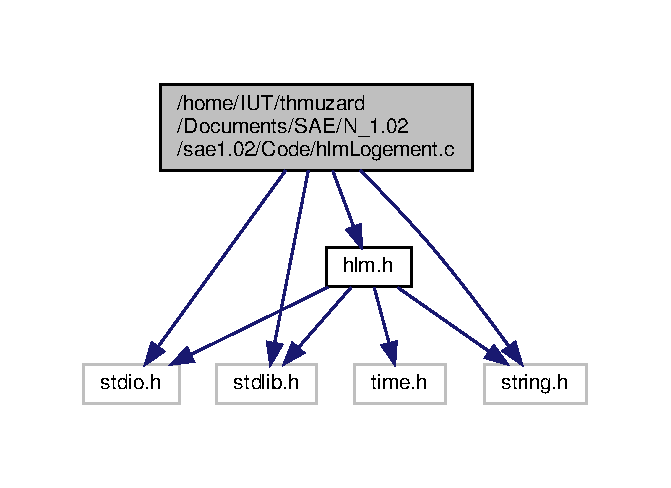
\includegraphics[width=322pt]{hlm_logement_8c__incl}
\end{center}
\end{figure}
\subsection*{Functions}
\begin{DoxyCompactItemize}
\item 
\hyperlink{struct_logement}{Logement} \hyperlink{hlm_logement_8c_a73f69309b57cab46c560476228f15da6}{lire\+Log} (F\+I\+LE $\ast$fe)
\begin{DoxyCompactList}\small\item\em Lit un logement dans le fichier. \end{DoxyCompactList}\item 
\hyperlink{struct_logement}{Logement} $\ast$ \hyperlink{hlm_logement_8c_afedc3d2e33c84f23d39c2a8207289974}{charge\+Logement} (F\+I\+LE $\ast$fe, int $\ast$nb\+Log)
\begin{DoxyCompactList}\small\item\em Charge dans le table, les éléments du fichier. \end{DoxyCompactList}\item 
void \hyperlink{hlm_logement_8c_afa143aab66778fe697a53485f9a73f38}{affichage\+Log} (\hyperlink{struct_logement}{Logement} t\+Log\mbox{[}$\,$\mbox{]}, int nb\+Log)
\begin{DoxyCompactList}\small\item\em Affiche les information des logements. \end{DoxyCompactList}\item 
int \hyperlink{hlm_logement_8c_ae42251f83bc9a022ea32c7204910009d}{supprime} (\hyperlink{struct_logement}{Logement} $\ast$t\+Log, int nb\+Log)
\begin{DoxyCompactList}\small\item\em Supprime un logement dans le tableau. \end{DoxyCompactList}\item 
int \hyperlink{hlm_logement_8c_a95c2be8a166e21b69c35624cad69f086}{recherche\+Dico} (\hyperlink{struct_logement}{Logement} $\ast$t\+Log, int nb\+Log, int value)
\begin{DoxyCompactList}\small\item\em recherche dans le tableau, un numéro de logement \end{DoxyCompactList}\item 
Booleen \hyperlink{hlm_logement_8c_a72f4f3b86e0afe012b41e360bb7f41ae}{num\+Log\+Existe} (\hyperlink{struct_logement}{Logement} $\ast$t\+Log, int value, int nb\+Log)
\begin{DoxyCompactList}\small\item\em Recherche si le numéro de logement existe ou non. \end{DoxyCompactList}\item 
\hyperlink{struct_logement}{Logement} $\ast$ \hyperlink{hlm_logement_8c_a7ae7af80a0f6bfeb8c30b2ef37fba7b2}{insertion\+Log} (\hyperlink{struct_logement}{Logement} $\ast$t\+Log, int $\ast$nb\+Log)
\begin{DoxyCompactList}\small\item\em Insère un logement dans le tableau. \end{DoxyCompactList}\item 
void \hyperlink{hlm_logement_8c_afcfd965c9496a6a0a57b60a4cb13fa8b}{affichage\+Log\+Dispo} (\hyperlink{struct_logement}{Logement} t\+Log\mbox{[}$\,$\mbox{]}, int nb\+Log)
\begin{DoxyCompactList}\small\item\em Affiche les logements disponible. \end{DoxyCompactList}\item 
void \hyperlink{hlm_logement_8c_a93abfc0f6ee8f58cf444aaf726133ae2}{sauvegarde\+Log} (\hyperlink{struct_logement}{Logement} t\+Log\mbox{[}$\,$\mbox{]}, int nb\+Log, F\+I\+LE $\ast$fe)
\begin{DoxyCompactList}\small\item\em Sauvegarde dans le fichier logements les ajout et suppression d\textquotesingle{}un logements. \end{DoxyCompactList}\end{DoxyCompactItemize}


\subsection{Detailed Description}
Ce fichier contiendra l\textquotesingle{}ensemble des fonction nécessaire au traitement des logement de la société 

\begin{DoxyAuthor}{Author}
V\+E\+R\+D\+I\+ER Nathan, M\+U\+Z\+A\+RD Thomas 
\end{DoxyAuthor}
\begin{DoxyDate}{Date}
14 janvier 2022
\end{DoxyDate}
Dans cette partit du programme, nous utilisons des tableaux pour exploité au mieux toute les notions vue en cours De plus, il était plus facile pour nous de faire les logement dans un tableau pour la simplicité du code

Ici, nous trions dans l\textquotesingle{}insertion du logement par numéro de logement 

\subsection{Function Documentation}
\mbox{\Hypertarget{hlm_logement_8c_afa143aab66778fe697a53485f9a73f38}\label{hlm_logement_8c_afa143aab66778fe697a53485f9a73f38}} 
\index{hlm\+Logement.\+c@{hlm\+Logement.\+c}!affichage\+Log@{affichage\+Log}}
\index{affichage\+Log@{affichage\+Log}!hlm\+Logement.\+c@{hlm\+Logement.\+c}}
\subsubsection{\texorpdfstring{affichage\+Log()}{affichageLog()}}
{\footnotesize\ttfamily void affichage\+Log (\begin{DoxyParamCaption}\item[{\hyperlink{struct_logement}{Logement}}]{t\+Log\mbox{[}$\,$\mbox{]},  }\item[{int}]{nb\+Log }\end{DoxyParamCaption})}



Affiche les information des logements. 


\begin{DoxyParams}{Parameters}
{\em \hyperlink{struct_logement}{Logement}} & t\+Log\mbox{[}\mbox{]} \+: Emplacement dans le tableau des logements \\
\hline
{\em nb\+Log} & nombre de logement \\
\hline
\end{DoxyParams}
\mbox{\Hypertarget{hlm_logement_8c_afcfd965c9496a6a0a57b60a4cb13fa8b}\label{hlm_logement_8c_afcfd965c9496a6a0a57b60a4cb13fa8b}} 
\index{hlm\+Logement.\+c@{hlm\+Logement.\+c}!affichage\+Log\+Dispo@{affichage\+Log\+Dispo}}
\index{affichage\+Log\+Dispo@{affichage\+Log\+Dispo}!hlm\+Logement.\+c@{hlm\+Logement.\+c}}
\subsubsection{\texorpdfstring{affichage\+Log\+Dispo()}{affichageLogDispo()}}
{\footnotesize\ttfamily void affichage\+Log\+Dispo (\begin{DoxyParamCaption}\item[{\hyperlink{struct_logement}{Logement}}]{t\+Log\mbox{[}$\,$\mbox{]},  }\item[{int}]{nb\+Log }\end{DoxyParamCaption})}



Affiche les logements disponible. 


\begin{DoxyParams}{Parameters}
{\em \hyperlink{struct_logement}{Logement}} & $\ast$t\+Log \+: Emplacement dans le tableau de logement \\
\hline
{\em nb\+Log} & nombre de logement \\
\hline
\end{DoxyParams}
\mbox{\Hypertarget{hlm_logement_8c_afedc3d2e33c84f23d39c2a8207289974}\label{hlm_logement_8c_afedc3d2e33c84f23d39c2a8207289974}} 
\index{hlm\+Logement.\+c@{hlm\+Logement.\+c}!charge\+Logement@{charge\+Logement}}
\index{charge\+Logement@{charge\+Logement}!hlm\+Logement.\+c@{hlm\+Logement.\+c}}
\subsubsection{\texorpdfstring{charge\+Logement()}{chargeLogement()}}
{\footnotesize\ttfamily \hyperlink{struct_logement}{Logement}$\ast$ charge\+Logement (\begin{DoxyParamCaption}\item[{F\+I\+LE $\ast$}]{fe,  }\item[{int $\ast$}]{nb\+Log }\end{DoxyParamCaption})}



Charge dans le table, les éléments du fichier. 


\begin{DoxyParams}{Parameters}
{\em $\ast$fe} & \+: fichier logement \\
\hline
{\em $\ast$nb\+Log} & nombre de logement \\
\hline
\end{DoxyParams}
\begin{DoxyReturn}{Returns}
Un tableau 
\end{DoxyReturn}
\mbox{\Hypertarget{hlm_logement_8c_a7ae7af80a0f6bfeb8c30b2ef37fba7b2}\label{hlm_logement_8c_a7ae7af80a0f6bfeb8c30b2ef37fba7b2}} 
\index{hlm\+Logement.\+c@{hlm\+Logement.\+c}!insertion\+Log@{insertion\+Log}}
\index{insertion\+Log@{insertion\+Log}!hlm\+Logement.\+c@{hlm\+Logement.\+c}}
\subsubsection{\texorpdfstring{insertion\+Log()}{insertionLog()}}
{\footnotesize\ttfamily \hyperlink{struct_logement}{Logement}$\ast$ insertion\+Log (\begin{DoxyParamCaption}\item[{\hyperlink{struct_logement}{Logement} $\ast$}]{t\+Log,  }\item[{int $\ast$}]{nb\+Log }\end{DoxyParamCaption})}



Insère un logement dans le tableau. 


\begin{DoxyParams}{Parameters}
{\em \hyperlink{struct_logement}{Logement}} & $\ast$t\+Log Emplacement dans le tableau des logements \\
\hline
{\em $\ast$nb\+Log} & nombre de logements dans le tableau \\
\hline
\end{DoxyParams}
\begin{DoxyReturn}{Returns}
Un tableau 
\end{DoxyReturn}
\mbox{\Hypertarget{hlm_logement_8c_a73f69309b57cab46c560476228f15da6}\label{hlm_logement_8c_a73f69309b57cab46c560476228f15da6}} 
\index{hlm\+Logement.\+c@{hlm\+Logement.\+c}!lire\+Log@{lire\+Log}}
\index{lire\+Log@{lire\+Log}!hlm\+Logement.\+c@{hlm\+Logement.\+c}}
\subsubsection{\texorpdfstring{lire\+Log()}{lireLog()}}
{\footnotesize\ttfamily \hyperlink{struct_logement}{Logement} lire\+Log (\begin{DoxyParamCaption}\item[{F\+I\+LE $\ast$}]{fe }\end{DoxyParamCaption})}



Lit un logement dans le fichier. 


\begin{DoxyParams}{Parameters}
{\em $\ast$fe} & \+: fichier des logements \\
\hline
\end{DoxyParams}
\begin{DoxyReturn}{Returns}
Un tableau 
\end{DoxyReturn}
\mbox{\Hypertarget{hlm_logement_8c_a72f4f3b86e0afe012b41e360bb7f41ae}\label{hlm_logement_8c_a72f4f3b86e0afe012b41e360bb7f41ae}} 
\index{hlm\+Logement.\+c@{hlm\+Logement.\+c}!num\+Log\+Existe@{num\+Log\+Existe}}
\index{num\+Log\+Existe@{num\+Log\+Existe}!hlm\+Logement.\+c@{hlm\+Logement.\+c}}
\subsubsection{\texorpdfstring{num\+Log\+Existe()}{numLogExiste()}}
{\footnotesize\ttfamily Booleen num\+Log\+Existe (\begin{DoxyParamCaption}\item[{\hyperlink{struct_logement}{Logement} $\ast$}]{t\+Log,  }\item[{int}]{value,  }\item[{int}]{nb\+Log }\end{DoxyParamCaption})}



Recherche si le numéro de logement existe ou non. 


\begin{DoxyParams}{Parameters}
{\em \hyperlink{struct_logement}{Logement}} & $\ast$t\+Log Emplacement dans le tableau des logements \\
\hline
{\em value} & Numéro de logement \\
\hline
{\em nb\+Log} & Nombre de logement \\
\hline
\end{DoxyParams}
\begin{DoxyReturn}{Returns}
Vrai ou Faux 
\end{DoxyReturn}
\mbox{\Hypertarget{hlm_logement_8c_a95c2be8a166e21b69c35624cad69f086}\label{hlm_logement_8c_a95c2be8a166e21b69c35624cad69f086}} 
\index{hlm\+Logement.\+c@{hlm\+Logement.\+c}!recherche\+Dico@{recherche\+Dico}}
\index{recherche\+Dico@{recherche\+Dico}!hlm\+Logement.\+c@{hlm\+Logement.\+c}}
\subsubsection{\texorpdfstring{recherche\+Dico()}{rechercheDico()}}
{\footnotesize\ttfamily int recherche\+Dico (\begin{DoxyParamCaption}\item[{\hyperlink{struct_logement}{Logement} $\ast$}]{t\+Log,  }\item[{int}]{nb\+Log,  }\item[{int}]{value }\end{DoxyParamCaption})}



recherche dans le tableau, un numéro de logement 


\begin{DoxyParams}{Parameters}
{\em \hyperlink{struct_logement}{Logement}} & $\ast$t\+Log Emplacement dans le tableau des logement \\
\hline
{\em nb\+Log} & nombre de logement  numéro de logement rechercher \\
\hline
\end{DoxyParams}
\begin{DoxyReturn}{Returns}
la position logement rechercher 
\end{DoxyReturn}
\mbox{\Hypertarget{hlm_logement_8c_a93abfc0f6ee8f58cf444aaf726133ae2}\label{hlm_logement_8c_a93abfc0f6ee8f58cf444aaf726133ae2}} 
\index{hlm\+Logement.\+c@{hlm\+Logement.\+c}!sauvegarde\+Log@{sauvegarde\+Log}}
\index{sauvegarde\+Log@{sauvegarde\+Log}!hlm\+Logement.\+c@{hlm\+Logement.\+c}}
\subsubsection{\texorpdfstring{sauvegarde\+Log()}{sauvegardeLog()}}
{\footnotesize\ttfamily void sauvegarde\+Log (\begin{DoxyParamCaption}\item[{\hyperlink{struct_logement}{Logement}}]{t\+Log\mbox{[}$\,$\mbox{]},  }\item[{int}]{nb\+Log,  }\item[{F\+I\+LE $\ast$}]{fe }\end{DoxyParamCaption})}



Sauvegarde dans le fichier logements les ajout et suppression d\textquotesingle{}un logements. 


\begin{DoxyParams}{Parameters}
{\em \hyperlink{struct_logement}{Logement}} & $\ast$t\+Log Tableau des logement \\
\hline
{\em nb\+Log} & nombre de logements \\
\hline
{\em $\ast$fe} & fichier des logements \\
\hline
\end{DoxyParams}
\mbox{\Hypertarget{hlm_logement_8c_ae42251f83bc9a022ea32c7204910009d}\label{hlm_logement_8c_ae42251f83bc9a022ea32c7204910009d}} 
\index{hlm\+Logement.\+c@{hlm\+Logement.\+c}!supprime@{supprime}}
\index{supprime@{supprime}!hlm\+Logement.\+c@{hlm\+Logement.\+c}}
\subsubsection{\texorpdfstring{supprime()}{supprime()}}
{\footnotesize\ttfamily int supprime (\begin{DoxyParamCaption}\item[{\hyperlink{struct_logement}{Logement} $\ast$}]{t\+Log,  }\item[{int}]{nb\+Log }\end{DoxyParamCaption})}



Supprime un logement dans le tableau. 


\begin{DoxyParams}{Parameters}
{\em \hyperlink{struct_logement}{Logement}} & $\ast$t\+Log \+: Emplacement dans le tableau des logements \\
\hline
{\em nb\+Log} & nombre de logement \\
\hline
\end{DoxyParams}
\begin{DoxyReturn}{Returns}
la position de l\textquotesingle{}élément 
\end{DoxyReturn}

\hypertarget{menu_8c}{}\section{/home/\+I\+U\+T/thmuzard/\+Documents/\+S\+A\+E/\+N\+\_\+1.02/sae1.02/\+Code/menu.c File Reference}
\label{menu_8c}\index{/home/\+I\+U\+T/thmuzard/\+Documents/\+S\+A\+E/\+N\+\_\+1.\+02/sae1.\+02/\+Code/menu.\+c@{/home/\+I\+U\+T/thmuzard/\+Documents/\+S\+A\+E/\+N\+\_\+1.\+02/sae1.\+02/\+Code/menu.\+c}}


Dans cette partie du programme, nous traitons les fonctions d\textquotesingle{}affichage des menu et l\textquotesingle{}aspect visuel du code. C\textquotesingle{}est ici que nous allons appellé toutes nos fonctions.  


{\ttfamily \#include \char`\"{}hlm.\+h\char`\"{}}\newline
Include dependency graph for menu.\+c\+:
\nopagebreak
\begin{figure}[H]
\begin{center}
\leavevmode
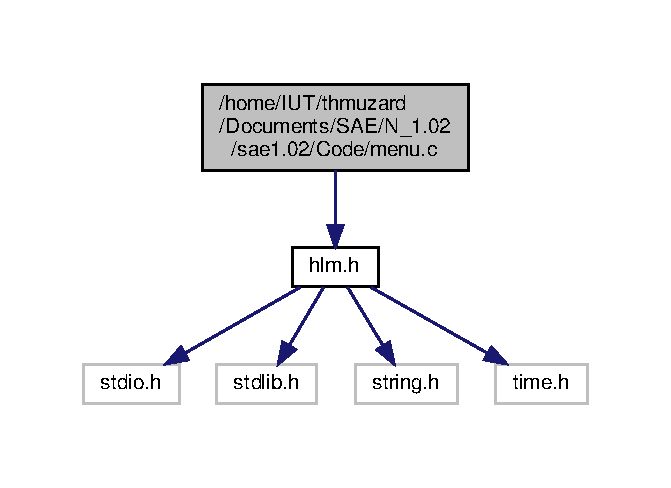
\includegraphics[width=322pt]{menu_8c__incl}
\end{center}
\end{figure}
\subsection*{Macros}
\begin{DoxyCompactItemize}
\item 
\mbox{\Hypertarget{menu_8c_a7b29335add3a553ed85d0e3ace85629c}\label{menu_8c_a7b29335add3a553ed85d0e3ace85629c}} 
\#define {\bfseries T\+A\+I\+L\+LE}~100
\end{DoxyCompactItemize}
\subsection*{Functions}
\begin{DoxyCompactItemize}
\item 
\mbox{\Hypertarget{menu_8c_af8eb04726a2e354f148a2d03d3b7c2a5}\label{menu_8c_af8eb04726a2e354f148a2d03d3b7c2a5}} 
void \hyperlink{menu_8c_af8eb04726a2e354f148a2d03d3b7c2a5}{affich\+Menu} (void)
\begin{DoxyCompactList}\small\item\em affichage des différente proposition du menu \end{DoxyCompactList}\item 
\mbox{\Hypertarget{menu_8c_a2a6e572b355984368bccd92a3f257013}\label{menu_8c_a2a6e572b355984368bccd92a3f257013}} 
void \hyperlink{menu_8c_a2a6e572b355984368bccd92a3f257013}{affich\+Menu\+Logement} (void)
\begin{DoxyCompactList}\small\item\em affichage des différente proposition du menu des logements \end{DoxyCompactList}\item 
\mbox{\Hypertarget{menu_8c_a26bc353bdb1ca2d0b715fbc7902afbaf}\label{menu_8c_a26bc353bdb1ca2d0b715fbc7902afbaf}} 
void \hyperlink{menu_8c_a26bc353bdb1ca2d0b715fbc7902afbaf}{affich\+Choix\+Trie\+Loca} (void)
\begin{DoxyCompactList}\small\item\em affichage des différente proposition de choix de trie des locataires \end{DoxyCompactList}\item 
\mbox{\Hypertarget{menu_8c_a5565a14a34b749c2c07599b27891f42a}\label{menu_8c_a5565a14a34b749c2c07599b27891f42a}} 
void \hyperlink{menu_8c_a5565a14a34b749c2c07599b27891f42a}{affich\+Menu\+Locataire} (void)
\begin{DoxyCompactList}\small\item\em affichage des différente proposition du menu des locataires \end{DoxyCompactList}\item 
\mbox{\Hypertarget{menu_8c_ad09f864d10061909d5d3b50b892a21a4}\label{menu_8c_ad09f864d10061909d5d3b50b892a21a4}} 
void \hyperlink{menu_8c_ad09f864d10061909d5d3b50b892a21a4}{affich\+Menu\+Dem\+Log} (void)
\begin{DoxyCompactList}\small\item\em affichage des différente proposition du menu des demandes de logements \end{DoxyCompactList}\item 
\mbox{\Hypertarget{menu_8c_ad16e5e62f3579a7048e6b981b172885e}\label{menu_8c_ad16e5e62f3579a7048e6b981b172885e}} 
void \hyperlink{menu_8c_ad16e5e62f3579a7048e6b981b172885e}{menu} (void)
\begin{DoxyCompactList}\small\item\em Menu général proposant une transitions sur toute les parties du code. \end{DoxyCompactList}\item 
\hyperlink{structmaillonloc}{Files} \hyperlink{menu_8c_aff8db4e369910a0e3cc7f42eca845add}{Menu\+Locataire} (\hyperlink{structmaillonloc}{Files} lc, int $\ast$nbL, \hyperlink{struct_logement}{Logement} t\+Log\mbox{[}$\,$\mbox{]}, int $\ast$nb\+Log, \hyperlink{structliste_dem}{Liste\+Dem} ld, int $\ast$nbD)
\begin{DoxyCompactList}\small\item\em Menu \hyperlink{struct_locataire}{Locataire} proposant les différents fonctionnalité proposé pour les locataires. \end{DoxyCompactList}\item 
\hyperlink{structmaillonloc}{Files} \hyperlink{menu_8c_a69bdc59a1d56a203005f12fa1578862b}{Menu\+Choix\+Trie} (\hyperlink{structmaillonloc}{Files} lc, int $\ast$nbL)
\begin{DoxyCompactList}\small\item\em Choix du trie des locataire dans un tableau de pointeur. \end{DoxyCompactList}\item 
void \hyperlink{menu_8c_a6ce592f9c0ed9073100ab23120608ff5}{Menu\+Logement} (\hyperlink{struct_logement}{Logement} t\+Log\mbox{[}$\,$\mbox{]}, int $\ast$nb\+Log)
\begin{DoxyCompactList}\small\item\em Choix des fonctionnalité des logements. \end{DoxyCompactList}\item 
\hyperlink{structliste_dem}{Liste\+Dem} \hyperlink{menu_8c_a3cad3605436db20a47369da7b4b3e13a}{Menu\+Dem\+Log} (\hyperlink{structliste_dem}{Liste\+Dem} ld, int $\ast$nbD)
\begin{DoxyCompactList}\small\item\em Choix des fonctionnalité proposé pour les demandes de logements. \end{DoxyCompactList}\item 
void \hyperlink{menu_8c_af3444c35a3ce252e06f2eb6865ba42d3}{sauvegarde\+Tout} (\hyperlink{structliste_dem}{Liste\+Dem} ld, char $\ast$fic\+Dem, int nbD, int nbL, \hyperlink{structmaillonloc}{Files} lc, char $\ast$fic\+Loc, \hyperlink{struct_logement}{Logement} $\ast$t\+Log, char $\ast$fic\+Log, int nb\+Log)
\begin{DoxyCompactList}\small\item\em Sauvegarde des les fichiers, les modification, ajout et suppression dans les fichiers appropriés. \end{DoxyCompactList}\end{DoxyCompactItemize}


\subsection{Detailed Description}
Dans cette partie du programme, nous traitons les fonctions d\textquotesingle{}affichage des menu et l\textquotesingle{}aspect visuel du code. C\textquotesingle{}est ici que nous allons appellé toutes nos fonctions. 

\begin{DoxyAuthor}{Author}
\+: V\+E\+R\+D\+I\+ER Nathan, M\+U\+Z\+A\+RD Thomas 
\end{DoxyAuthor}
\begin{DoxyDate}{Date}
\+: 14 janvier 2022 
\end{DoxyDate}


\subsection{Function Documentation}
\mbox{\Hypertarget{menu_8c_a69bdc59a1d56a203005f12fa1578862b}\label{menu_8c_a69bdc59a1d56a203005f12fa1578862b}} 
\index{menu.\+c@{menu.\+c}!Menu\+Choix\+Trie@{Menu\+Choix\+Trie}}
\index{Menu\+Choix\+Trie@{Menu\+Choix\+Trie}!menu.\+c@{menu.\+c}}
\subsubsection{\texorpdfstring{Menu\+Choix\+Trie()}{MenuChoixTrie()}}
{\footnotesize\ttfamily \hyperlink{structmaillonloc}{Files} Menu\+Choix\+Trie (\begin{DoxyParamCaption}\item[{\hyperlink{structmaillonloc}{Files}}]{lc,  }\item[{int $\ast$}]{nbL }\end{DoxyParamCaption})}



Choix du trie des locataire dans un tableau de pointeur. 


\begin{DoxyParams}{Parameters}
{\em Files} & lc \+: file des locataire \\
\hline
{\em $\ast$nbL} & nombre de locataire \\
\hline
\end{DoxyParams}
\begin{DoxyReturn}{Returns}
Une file 
\end{DoxyReturn}
\mbox{\Hypertarget{menu_8c_a3cad3605436db20a47369da7b4b3e13a}\label{menu_8c_a3cad3605436db20a47369da7b4b3e13a}} 
\index{menu.\+c@{menu.\+c}!Menu\+Dem\+Log@{Menu\+Dem\+Log}}
\index{Menu\+Dem\+Log@{Menu\+Dem\+Log}!menu.\+c@{menu.\+c}}
\subsubsection{\texorpdfstring{Menu\+Dem\+Log()}{MenuDemLog()}}
{\footnotesize\ttfamily \hyperlink{structliste_dem}{Liste\+Dem} Menu\+Dem\+Log (\begin{DoxyParamCaption}\item[{\hyperlink{structliste_dem}{Liste\+Dem}}]{ld,  }\item[{int $\ast$}]{nbD }\end{DoxyParamCaption})}



Choix des fonctionnalité proposé pour les demandes de logements. 


\begin{DoxyParams}{Parameters}
{\em Liste\+Dem} & ld \+: Liste des demandeurs \\
\hline
{\em $\ast$nbD} & nombre demandeurs \\
\hline
\end{DoxyParams}
\begin{DoxyReturn}{Returns}
une liste 
\end{DoxyReturn}
\mbox{\Hypertarget{menu_8c_aff8db4e369910a0e3cc7f42eca845add}\label{menu_8c_aff8db4e369910a0e3cc7f42eca845add}} 
\index{menu.\+c@{menu.\+c}!Menu\+Locataire@{Menu\+Locataire}}
\index{Menu\+Locataire@{Menu\+Locataire}!menu.\+c@{menu.\+c}}
\subsubsection{\texorpdfstring{Menu\+Locataire()}{MenuLocataire()}}
{\footnotesize\ttfamily \hyperlink{structmaillonloc}{Files} Menu\+Locataire (\begin{DoxyParamCaption}\item[{\hyperlink{structmaillonloc}{Files}}]{lc,  }\item[{int $\ast$}]{nbL,  }\item[{\hyperlink{struct_logement}{Logement}}]{t\+Log\mbox{[}$\,$\mbox{]},  }\item[{int $\ast$}]{nb\+Log,  }\item[{\hyperlink{structliste_dem}{Liste\+Dem}}]{ld,  }\item[{int $\ast$}]{nbD }\end{DoxyParamCaption})}



Menu \hyperlink{struct_locataire}{Locataire} proposant les différents fonctionnalité proposé pour les locataires. 


\begin{DoxyParams}{Parameters}
{\em Files} & lc \+: File des locataires \\
\hline
{\em $\ast$nbL} & nombre de locataire \\
\hline
{\em \hyperlink{struct_logement}{Logement}} & $\ast$t\+Log \+: Tableau des logements \\
\hline
{\em $\ast$nb\+Log} & nombre de logement \\
\hline
{\em Liste\+Dem} & ld \+: Liste des demandeurs \\
\hline
{\em $\ast$nbD} & nombre de demandeurs \\
\hline
\end{DoxyParams}
\begin{DoxyReturn}{Returns}
Une file 
\end{DoxyReturn}
\mbox{\Hypertarget{menu_8c_a6ce592f9c0ed9073100ab23120608ff5}\label{menu_8c_a6ce592f9c0ed9073100ab23120608ff5}} 
\index{menu.\+c@{menu.\+c}!Menu\+Logement@{Menu\+Logement}}
\index{Menu\+Logement@{Menu\+Logement}!menu.\+c@{menu.\+c}}
\subsubsection{\texorpdfstring{Menu\+Logement()}{MenuLogement()}}
{\footnotesize\ttfamily void Menu\+Logement (\begin{DoxyParamCaption}\item[{\hyperlink{struct_logement}{Logement}}]{t\+Log\mbox{[}$\,$\mbox{]},  }\item[{int $\ast$}]{nb\+Log }\end{DoxyParamCaption})}



Choix des fonctionnalité des logements. 


\begin{DoxyParams}{Parameters}
{\em \hyperlink{struct_logement}{Logement}} & $\ast$t\+Log \+: tableau des logements \\
\hline
{\em $\ast$nb\+Log} & nombre de logement \\
\hline
\end{DoxyParams}
\mbox{\Hypertarget{menu_8c_af3444c35a3ce252e06f2eb6865ba42d3}\label{menu_8c_af3444c35a3ce252e06f2eb6865ba42d3}} 
\index{menu.\+c@{menu.\+c}!sauvegarde\+Tout@{sauvegarde\+Tout}}
\index{sauvegarde\+Tout@{sauvegarde\+Tout}!menu.\+c@{menu.\+c}}
\subsubsection{\texorpdfstring{sauvegarde\+Tout()}{sauvegardeTout()}}
{\footnotesize\ttfamily void sauvegarde\+Tout (\begin{DoxyParamCaption}\item[{\hyperlink{structliste_dem}{Liste\+Dem}}]{ld,  }\item[{char $\ast$}]{fic\+Dem,  }\item[{int}]{nbD,  }\item[{int}]{nbL,  }\item[{\hyperlink{structmaillonloc}{Files}}]{lc,  }\item[{char $\ast$}]{fic\+Loc,  }\item[{\hyperlink{struct_logement}{Logement} $\ast$}]{t\+Log,  }\item[{char $\ast$}]{fic\+Log,  }\item[{int}]{nb\+Log }\end{DoxyParamCaption})}



Sauvegarde des les fichiers, les modification, ajout et suppression dans les fichiers appropriés. 


\begin{DoxyParams}{Parameters}
{\em Liste\+Dem} & ld Liste des demandeurs \\
\hline
{\em $\ast$fic\+Dem} & nom fichier demandeur \\
\hline
{\em nbD} & nombre de demandeur \\
\hline
{\em int} & nbL nombre de locataire \\
\hline
{\em Files} & lc File des locataires \\
\hline
{\em $\ast$fic\+Loc} & fichier des locataire \\
\hline
{\em nb\+Log} & nombre de logement \\
\hline
{\em \hyperlink{struct_logement}{Logement}} & $\ast$t\+Log tableau des logements \\
\hline
{\em $\ast$fic\+Log} & fichier des logements \\
\hline
\end{DoxyParams}

%--- End generated contents ---

% Index
\backmatter
\newpage
\phantomsection
\clearemptydoublepage
\addcontentsline{toc}{chapter}{Index}
\printindex

\end{document}
